\section{Phase 1: Einfache und Fortgeschrittene Netzwerkmodelle}
\label{subsec:Basic_Advanced_Models}

In diesem Abschnitt werden die Ergebnisse der drei verschiedenen Ansätze zur Optimierung des DC-DC-Wandlers vorgestellt: die Bayesianische Optimierung sowie die kleinen und großen DDPG-Netzwerkmodelle. Die Belohnungen, die mit jeder Konfiguration erzielt wurden, bieten einen Einblick in die Effektivität jedes Ansatzes.

\paragraph{Hyperparameter}

\begin{table}[htbp]
\centering
\caption{Erweiterter Vergleich der Hyperparameter für das kleine und große DDPG-Modell unter Einbeziehung des Parameterraums}
\label{tab:extended_hyperparameters}
\begin{tabular}{lcc}
\hline
\textbf{Parameter} & \textbf{Kleines Modell} & \textbf{Großes Modell} \\
\hline
ALPHA & 0.001 & 0.0001 \\
WORKER & 12 & 12 \\
ITERATION & 1 & 1 \\
STEPS & 2000 & 20000 \\
BATCH\_SIZE & 72 & 250 \\
EXPLOITATION & 10 & 10 \\
LAYERS & 2 & 12 \\
LAYER\_1 & 158 & 158 \\
LAYER\_2 & 52 & 52 \\
NOISE & 0.3 & 0.45 \\
GAMMA & 0.0 & 0.0 \\
\textbf{Kp-Bereich} & 0 bis 10 & 0 bis 10 \\
\textbf{Ki-Bereich} & 0.0 bis 1.0 & 0.0 bis 1.0 \\
\textbf{Kd-Bereich} & 0.0 bis 0.2 & 0.0 bis 0.2 \\
\hline
\end{tabular}
\end{table}

\begin{figure}[htbp]
\centering
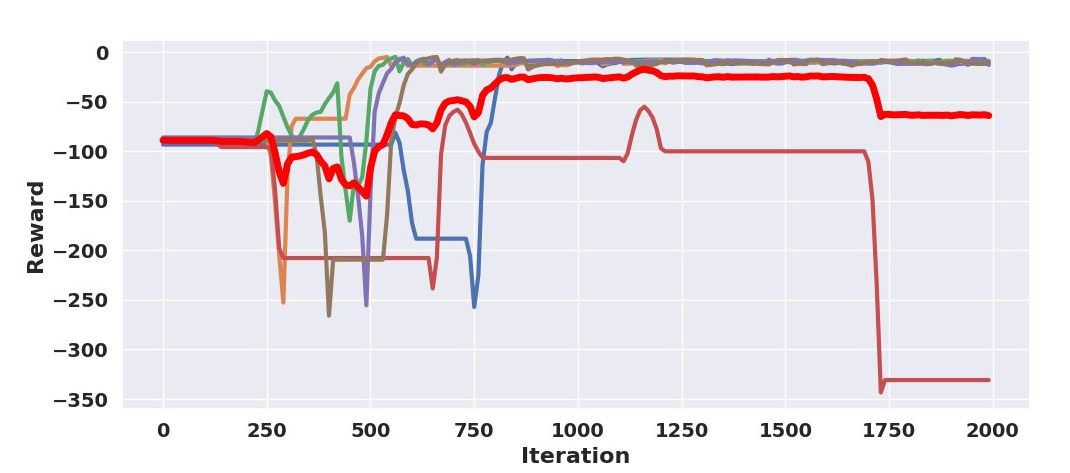
\includegraphics[width=0.7\textwidth]{4Ergebnisse/Phasen/1Phase/1Q_klein_epoch.png}
\caption{Belohnungsentwicklung über die Zeit für das kleine DDPG-Modell.}
\end{figure}

\begin{figure}[htbp]
\centering
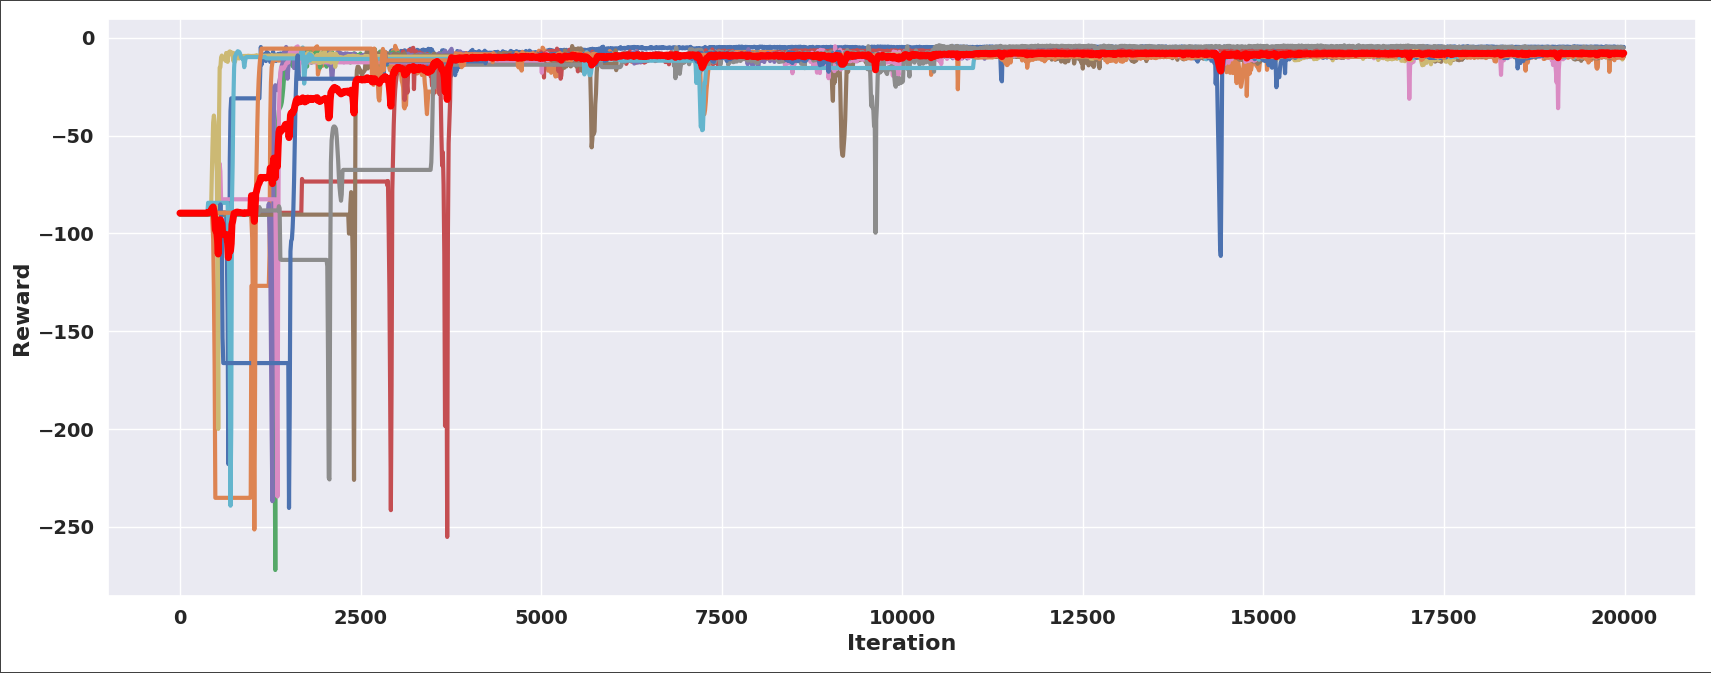
\includegraphics[width=0.92\textwidth,  trim=10px 10px 10px 10px, clip]{4Ergebnisse/Phasen/1Phase//1R_gross_epoch.png}
\caption{Belohnungsentwicklung über die Zeit für das große DDPG-Modell.}
\end{figure}


\begin{table}[htbp]
\centering
\caption{Vergleich der Ergebnisse verschiedener Modelle}
\label{tab:model_comparison}
\begin{tabular}{|c|c|c|}
\hline
\textbf{Modell} & \textbf{Ergebnis} & \textbf{Parameter} \\
\hline
Bayesian Optimization & -3.63 & 
\begin{tabular}[c]{@{}c@{}}Induktivität: 5.0e-3\\ Kapazität: 10.0e-6\\ Kp: 3.9250\\ Ki: 0.8521\\ Kd: 0.0139\end{tabular} \\
\hline
Kleines DDPG-Modell & -3.9098 & 
\begin{tabular}[c]{@{}c@{}}Induktivität: 5.0e-3\\ Kapazität: 10.0e-6\\ Kp: 2.4306\\ Ki: 0.6766\\ Kd: 0.0094\end{tabular} \\
\hline
Großes DDPG-Modell & -3.4217 & 
\begin{tabular}[c]{@{}c@{}}Induktivität: 5.0e-3\\ Kapazität: 10.0e-6\\ Kp: 3.4217\\ Ki: 0.6777\\ Kd: 0.0127\end{tabular} \\
\hline
\end{tabular}
\end{table}


\begin{figure}[htbp]
\centering
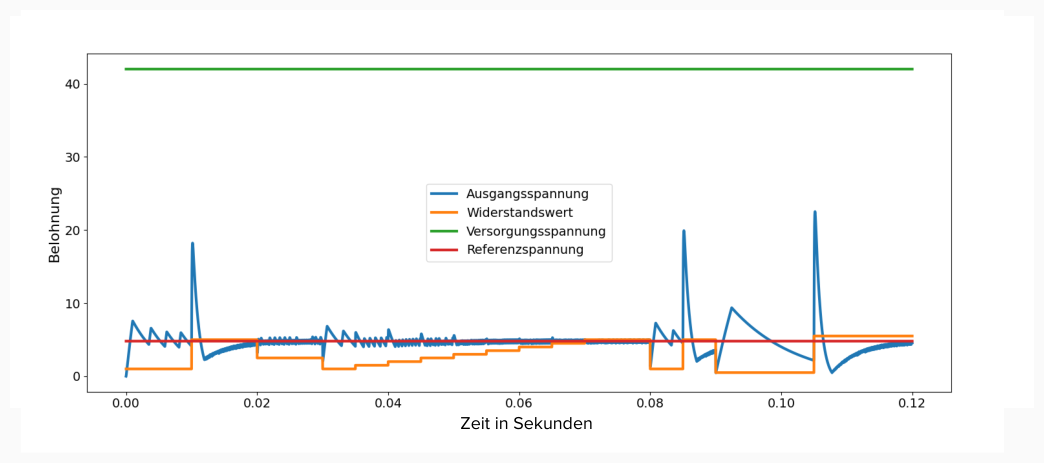
\includegraphics[width=0.99\textwidth, trim=10px 10px 10px 10px, clip]{4Ergebnisse/Phasen/1Phase/1S_small_search_space_bayes.png}
\caption{Darstellung des Regelungsverhaltens eines durch Bayes'sche Optimierung eingestellten PID-gesteuerten DC-DC-Konverters. Die Grafik zeigt die Belohnungsentwicklung über die Zeit und reflektiert die Anpassung der Ausgangsspannung (blau) an die Referenzspannung (rot) unter Berücksichtigung der Versorgungsspannung (grün) und des Widerstandswertes (orange). Die Ergebnisse verdeutlichen die Effektivität der Bayes'schen Optimierung bei der Feinabstimmung des Reglers für eine stabile Spannungsregelung.}
\label{fig:bayesian_optimization_pid_control}
\end{figure}
%
\begin{figure}[htbp]
\centering
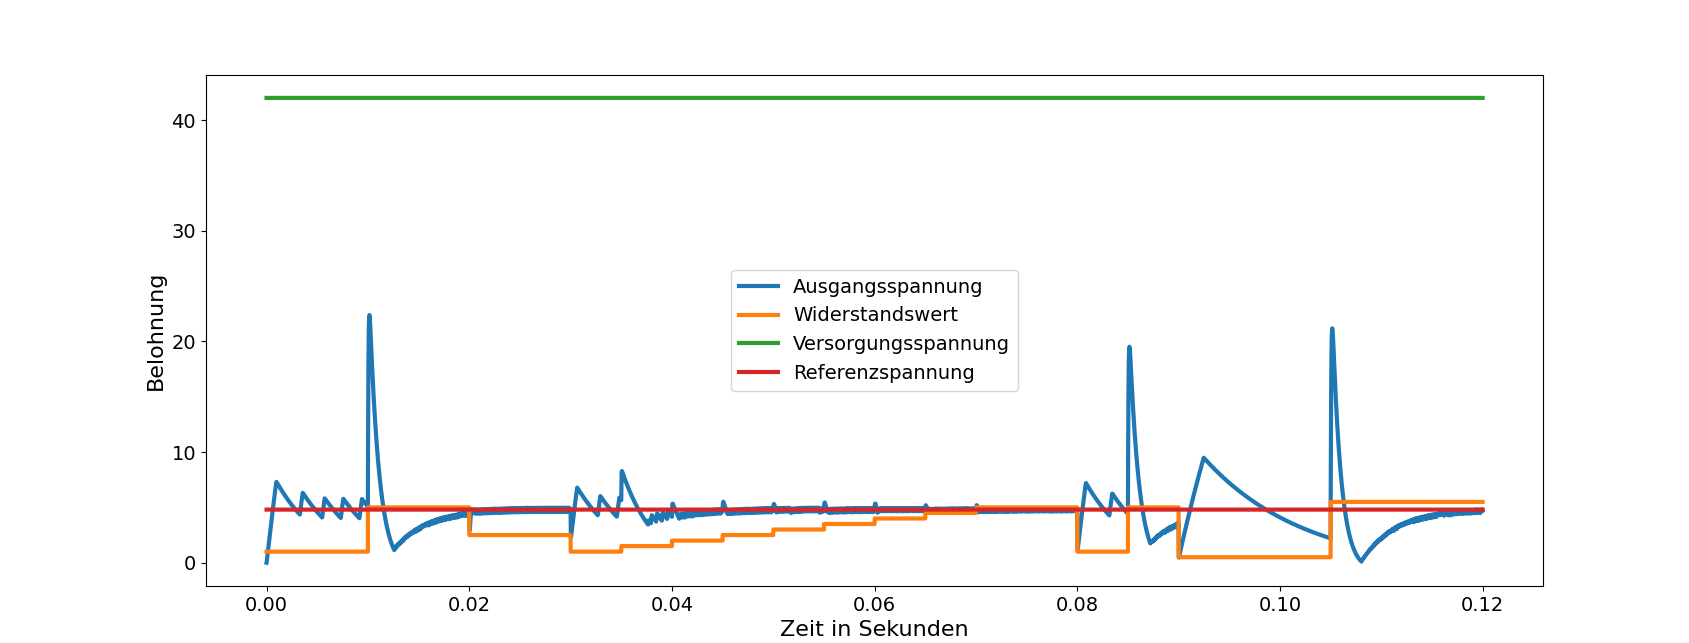
\includegraphics[width=0.99\textwidth]{4Ergebnisse/Phasen/1Phase//1T_small_search_space_small_net_dcdc.png}
\caption{Regelungsverhaltens über die Zeit für das kleine DDPG-Modell.}
\label{fig:small_ddpg_results}
\end{figure}
%
\begin{figure}[htbp]
\centering
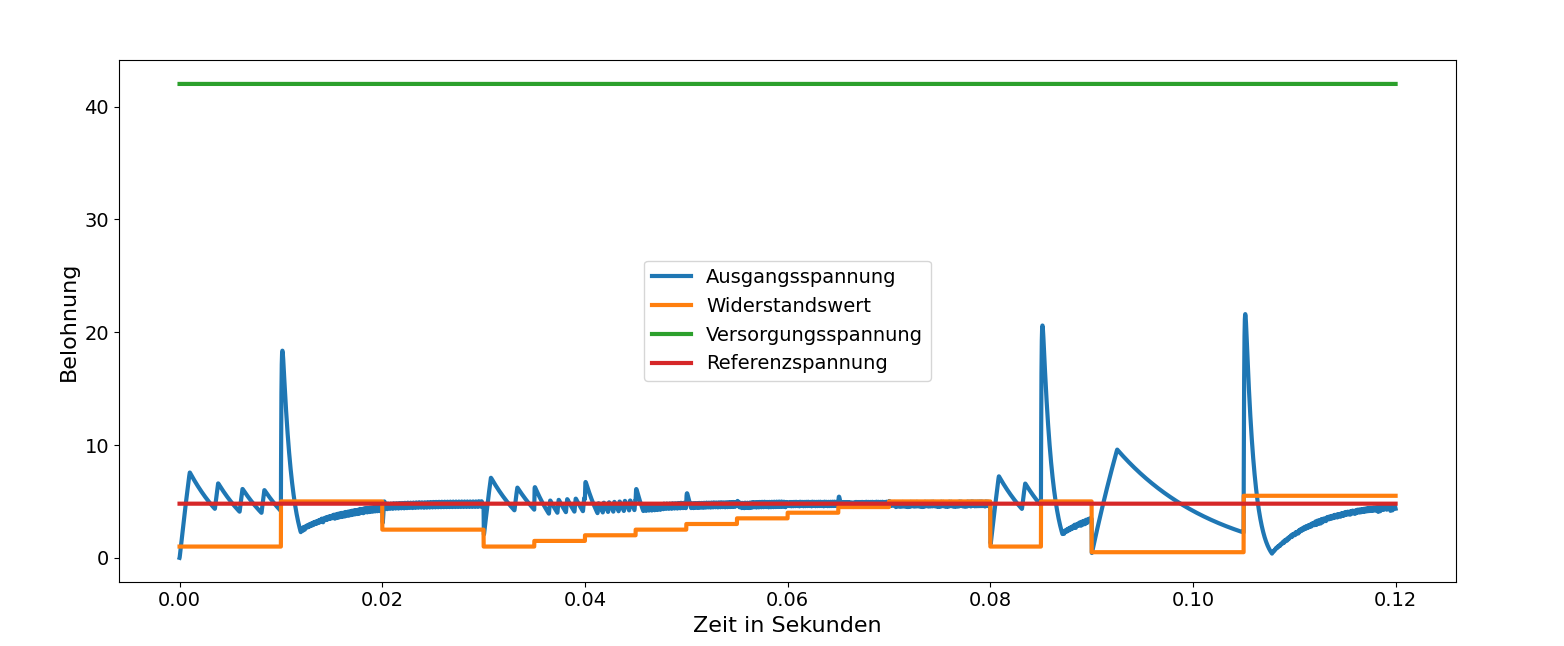
\includegraphics[width=0.99\textwidth]{4Ergebnisse/Phasen/1Phase//1U_big_net_dcdc.png}
\caption{Regelungsverhaltens über die Zeit für das große DDPG-Modell.}
\label{fig:large_ddpg_results}
\end{figure}

Die Abbildungen \ref{fig:bayesian_optimization_results}, \ref{fig:small_ddpg_results} und \ref{fig:large_ddpg_results} zeigen die jeweiligen Belohnungen, die durch die unterschiedlichen Optimierungsverfahren erzielt wurden.

\paragraph{Analyse der Ergebnisse: Leistungsvergleich der Optimierungsansätze}
Bei der Betrachtung der erzielten Ergebnisse aus den verschiedenen Optimierungsansätzen wird deutlich, dass sich die Leistungsdifferenzen vor allem im Belohnungswert (Reward) widerspiegeln. Alle drei Ansätze - Bayesianische Optimierung, kleines und großes DDPG-Modell - waren in der Lage, eine optimale oder nahezu optimale Lösung für die gestellte Aufgabe zu finden, wobei die Unterschiede in den tatsächlichen Spannungsverläufen minimal waren.

Interessanterweise zeigte das kleinere DDPG-Modell die geringste Leistung, was sich sowohl in niedrigeren Belohnungswerten als auch in einer weniger stabilen Konvergenz äußerte. Im Gegensatz dazu erreichte das große DDPG-Modell die besten Belohnungswerte, wobei alle Modelle eine gewisse Leichtigkeit bei der Konvergenz zeigten. Die Bayesianische Optimierung lag in ihrer Leistung dazwischen.

\paragraph{Synthese der Ergebnisse}

Interessanterweise zeigen sowohl die Bayesianische Optimierung als auch die DDPG-Modelle in ihren jeweiligen Anwendungen bemerkenswerte Übereinstimmungen in ihren Ergebnissen. Diese Konsistenz unterstreicht die Robustheit unserer Methoden und die Verlässlichkeit der erzielten Optimierungen. Trotz der unterschiedlichen Herangehensweisen und Techniken, die bei diesen beiden Methoden zum Einsatz kommen, konvergieren ihre Ergebnisse hin zu ähnlichen Lösungen. Dies deutet darauf hin, dass beide Ansätze effektiv die kritischen Bereiche des Parameterraums identifizieren und optimieren, was ein zentrales Ziel unserer Forschung ist.
